% Chapter 5. Where the hooks go. Every one of these is a place you can say no.
\documentclass[tikz,border=6pt]{standalone}
% Shared look for every TikZ figure in the book.
% Colours match book/preamble.tex exactly. Change both or neither.

\usepackage{tikz}
\usepackage{xcolor}
\usepackage{amsmath}
\IfFileExists{libertinus.sty}{\usepackage[mono=false]{libertinus}}{}
\IfFileExists{inconsolata.sty}{\usepackage[varqu,varl,scaled=0.95]{inconsolata}}{}

\usetikzlibrary{
  arrows.meta, positioning, calc, fit, backgrounds, shapes.geometric,
  shapes.misc, decorations.pathreplacing, decorations.pathmorphing,
  patterns, chains, matrix, shadows.blur
}

\definecolor{ink}{HTML}{15181D}
\definecolor{muted}{HTML}{5B6472}
\definecolor{rule}{HTML}{C9CED6}
\definecolor{wash}{HTML}{F4F5F7}
\definecolor{accent}{HTML}{0F5C8C}
\definecolor{accentsoft}{HTML}{E7F0F6}
\definecolor{warm}{HTML}{B4531A}
\definecolor{warmsoft}{HTML}{FBF0E7}
\definecolor{good}{HTML}{2C6E49}
\definecolor{goodsoft}{HTML}{E9F2EC}
\definecolor{danger}{HTML}{9B2226}
\definecolor{dangersoft}{HTML}{FAECEC}

\tikzset{
  font=\sffamily\small,
  >={Stealth[length=5pt, width=4pt]},
  %
  box/.style={
    draw=rule, line width=0.8pt, fill=wash, rounded corners=2pt,
    inner sep=7pt, align=center, text=ink, minimum height=9mm,
  },
  boxa/.style={box, draw=accent, fill=accentsoft},
  boxg/.style={box, draw=good,   fill=goodsoft},
  boxw/.style={box, draw=warm,   fill=warmsoft},
  boxd/.style={box, draw=danger, fill=dangersoft},
  %
  lane/.style={draw=rule, line width=0.7pt, fill=white, rounded corners=2pt,
               inner sep=6pt, align=center, minimum width=26mm},
  %
  flow/.style={draw=accent, line width=1.0pt, ->},
  flowback/.style={flow, densely dashed},
  flowmuted/.style={draw=muted, line width=0.8pt, ->},
  lifeline/.style={draw=rule, line width=0.7pt, densely dotted},
  %
  lbl/.style={font=\sffamily\scriptsize, text=muted, inner sep=2pt},
  lblink/.style={font=\sffamily\scriptsize, text=ink, inner sep=2pt},
  tag/.style={font=\ttfamily\scriptsize, text=accent, inner sep=2pt,
              fill=white, inner xsep=3pt},
  note/.style={font=\sffamily\scriptsize\itshape, text=muted, align=left},
  %
  band/.style={draw=none, rounded corners=1pt},
  tick/.style={draw=muted, line width=0.6pt},
}

% A horizontal timeline bar segment: \barseg{x0}{x1}{y}{colour}{label}
\newcommand{\barseg}[5]{%
  \fill[#4, rounded corners=1pt] (#1,#3-0.16) rectangle (#2,#3+0.16);
  \node[lbl, text=white, font=\sffamily\scriptsize\bfseries]
       at ({(#1+#2)/2},#3) {#5};
}

\begin{document}
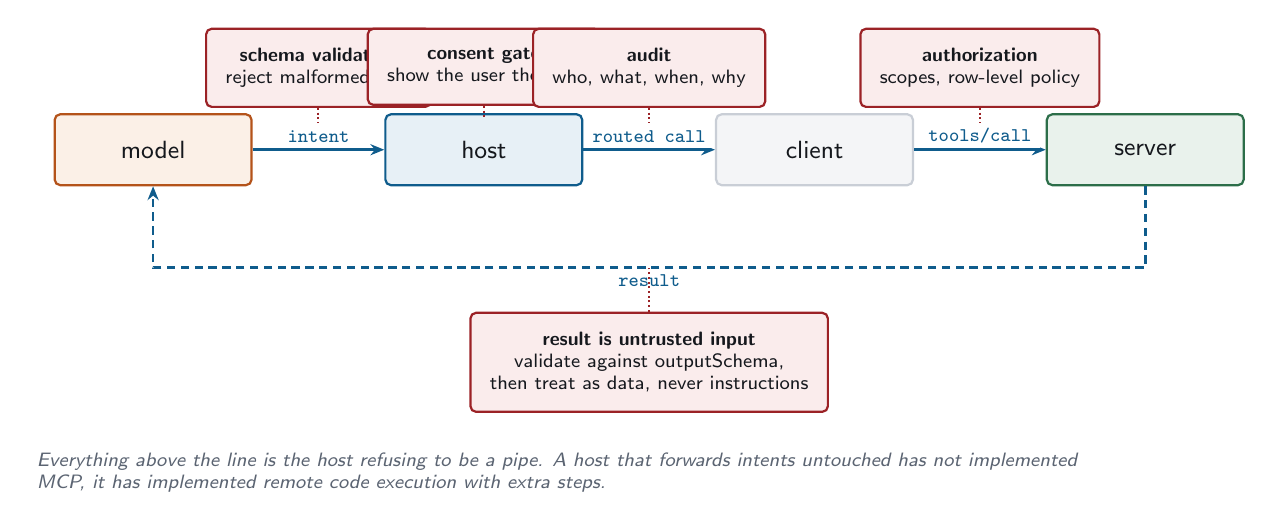
\begin{tikzpicture}[x=1cm, y=1cm]

  \node[boxw, minimum width=25mm] (model) at (0,0) {model};
  \node[boxa, minimum width=25mm] (host)  at (4.2,0) {host};
  \node[box,  minimum width=25mm] (client) at (8.4,0) {client};
  \node[boxg, minimum width=25mm] (server) at (12.6,0) {server};

  % outbound
  \draw[flow] (model) -- node[tag, above] {intent} (host);
  \draw[flow] (host)  -- node[tag, above] {routed call} (client);
  \draw[flow] (client) -- node[tag, above] {tools/call} (server);

  % return
  \draw[flowback] (server) -- ++(0,-1.5) -- node[tag, below] {result} ($(model)+(0,-1.5)$) -- (model);

  % --- the hook points ---------------------------------------------------
  \newcommand{\hook}[3]{%
    \node[boxa, draw=danger, fill=dangersoft, minimum width=27mm,
          align=center, font=\sffamily\scriptsize, anchor=north]
      (#1) at (#2,1.55) {#3};
  }

  \hook{h1}{2.1}{\textbf{schema validation}\\reject malformed args}
  \hook{h2}{4.2}{\textbf{consent gate}\\show the user the args}
  \hook{h3}{6.3}{\textbf{audit}\\who, what, when, why}
  \hook{h4}{10.5}{\textbf{authorization}\\scopes, row-level policy}

  \draw[draw=danger, line width=0.7pt, densely dotted] (h1.south) -- (2.1,0.35);
  \draw[draw=danger, line width=0.7pt, densely dotted] (h2.south) -- (4.2,0.4);
  \draw[draw=danger, line width=0.7pt, densely dotted] (h3.south) -- (6.3,0.35);
  \draw[draw=danger, line width=0.7pt, densely dotted] (h4.south) -- (10.5,0.35);

  % --- the return-path hook ----------------------------------------------
  \node[boxa, draw=danger, fill=dangersoft, minimum width=34mm, align=center,
        font=\sffamily\scriptsize] (h5) at (6.3,-2.7)
    {\textbf{result is untrusted input}\\validate against outputSchema,\\
     then treat as data, never instructions};
  \draw[draw=danger, line width=0.7pt, densely dotted] (h5.north) -- (6.3,-1.5);

  \node[note, anchor=west, align=left, text=muted] at (-1.6,-4.1)
    {Everything above the line is the host refusing to be a pipe. A host that
     forwards intents untouched has not implemented\\MCP, it has implemented
     remote code execution with extra steps.};

\end{tikzpicture}
\end{document}
